\section{Λειτουργικά Συστήματα}
\label{sec:os}
Σύμφωνα με το \cite{stallings}: Τα \textbf{Λειτουργικά Συστήματα} (εν συντομία \textbf{ΛΣ}) είναι προγράμματα που ελέγχουν την εκτέλεση προγραμμάτων εφαρμογών και δρουν ως διεπαφή ανάμεσα στις εφαρμογές και το υλικό του υπολογιστή. Θα λέγαμε ότι έχουν τρεις στόχους:
\begin{itemize}
	\item \textbf{Ευκολία:} Τα ΛΣ κάνουν ευκολότερη τη χρήση ενός υπολογιστή.
	\item \textbf{Αποτελεσματικότητα:} Τα ΛΣ επιτρέπουν την αποτελεσματική χρήση των πόρων ενός υπολογιστικού συστήματος.
	\item \textbf{Ικανότητα Εξέλιξης:} Τα ΛΣ πρέπει να είναι κατασκευασμένα με τέτοιο τρόπο, ώστε να επιτρέπουν την αποτελεσματική ανάπτυξη, τον έλεγχο και την εισαγωγή νέων λειτουργιών συστήματος, χωρίς να παρεμβαίνουν στην παροχή υπηρεσιών.
\end{itemize}

\subsection{Το ΛΣ ως Διεπαφή Χρήστη/Υπολογιστή}
Ένας υπολογιστής είναι ένα σύστημα που αποτελείται από το υλικό (hardware) και το λογισμικό (software). Το υλικό είναι ο φυσικός εξοπλισμός (οθόνες, μνήμες, εκτυπωτές κτλ) ενώ το λογισμικό είναι μια συλλογή προγραμμάτων που επιτρέπουν στο υλικό να λειτουργεί \cite{forouzan}. Το λογισμικό διαιρείται σε 2 κατηγορίες: στα προγράμματα εφαρμογών και στα λειτουργικά συστήματα. Το υλικό και το λογισμικό που αποτελούν ένα υπολογιστικό σύστημα μπορεί να αναπαρασταθεί από μια ιεραρχική δομή ή μια δομή επιπέδων, όπως φαίνεται στο Σχήμα \ref{fig:os_hierarchy}.
\begin{figure}[t]
	\centering
	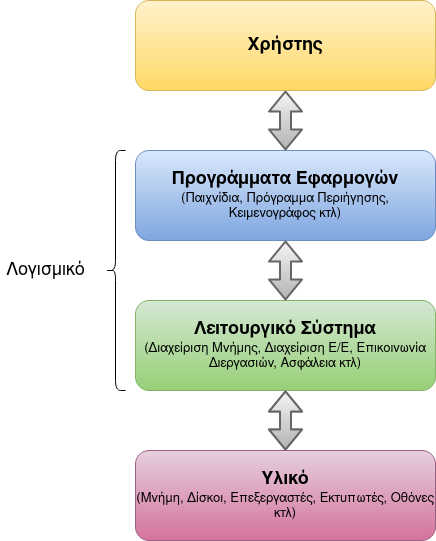
\includegraphics[scale=0.6]{./images/chapter2/OS_hierarchy.png}
	\caption{Δομή Υλικού και Λογισμικού Υπολογιστή}
	\label{fig:os_hierarchy}
\end{figure}

Το ΛΣ, επομένως, <<κάθεται>> ανάμεσα στο υλικό και στις εφαρμογές που χρησιμοποιεί ο χρήστης ο οποίος συνήθως δεν ενδιαφέρεται για λεπτομέρειες του υλικού του υπολογιστή. Δρα, δηλαδή, ως ένας διαμεσολαβητής που διευκολύνει την επικοινωνία του χρήστη με τον υπολογιστή χωρίς ο πρώτος να χρειάζεται να γνωρίζει την γλώσσα του τελευταίου, ενώ είναι υπεύθυνο για την ομαλή λειτουργία των προγραμμάτων εφαρμογών. Για παράδειγμα, προκειμένου να εμφανιστεί το κείμενο <<Χαίρε Κόσμε>> στην οθόνη, πρέπει μερικές εκατοντάδες πίξελ να λειτουργήσουν σε συγκεκριμένες θέσεις. Αυτό μπορεί να γίνει με το να διαβάζει κανείς τις προδιαγραφές του υλικού και να γράψει κώδικα που χειρίζεται τα σωστά μπιτς στην μνήμη κάτι που είναι αρκετά επίπονο. Οι περισσότεροι χρήστες όμως θέλουν απλά να γράψουν την εντολή \texttt{print("Hello World")} χωρίς να νοιαστούν για περαιτέρω λεπτομέρειες. Εκεί είναι που μπαίνει το ΛΣ για να δώσει λύση \cite{elements_of_computing}.

Πιο αναλυτικά, μερικές από τις περιοχές στις οποίες το ΛΣ παρέχει υπηρεσίες περιγράφονται παρακάτω σύμφωνα με το \cite{stallings}:

\begin{itemize}
	\item \textbf{Στην ανάπτυξη προγραμμάτων:} Το ΛΣ παρέχει πληθώρα υπηρεσιών, όπως επεξεργαστές κειμένου και διορθωτές λαθών (debuggers), προκειμένου να βοηθήσει τον προγραμματιστή στην ανάπτυξη εφαρμογών. Συνήθως, οι υπηρεσίες αυτές έχουν τη μορφή βοηθητικών προγραμμάτων, τα οποία αν και δεν αποτελούν αυστηρά τμήμα του πυρήνα του λειτουργικού συστήματος, παρέχονται μαζί με το ΛΣ και αναφέρονται ως εργαλεία ανάπτυξης προγραμμάτων εφαρμογών.
	\item \textbf{Στην εκτέλεση προγραμμάτων:} Για την εκτέλεση ενός προγράμματος απαιτείται πλήθος βημάτων. Εντολές και δεδομένα πρέπει να φορτωθούν στην κύρια μνήμη, συσκευές Εισόδου/Εξόδου (Ε/Ε) και αρχεία πρέπει να αρχικοποιηθούν και διάφοροι άλλοι πόροι πρέπει να ετοιμαστούν. Το ΛΣ διαχειρίζεται αυτές τις υποχρεώσεις χρονοδρομολόγησης για λογαριασμό του χρήστη.
	\item \textbf{Στην πρόσβαση σε συσκευές Εισόδου/Εξόδου(Ε/Ε):} Κάθε συσκευή Ε/Ε απαιτεί το δικό της ιδιαίτερο σύνολο εντολών ή σημάτων ελέγχου για τη λειτουργία της. Το ΛΣ παρέχει ενιαία διεπαφή που αποκρύπτει αυτές τις λεπτομέρειες, έτσι ώστε οι προγραμματιστές να έχουν πρόσβαση σε τέτοιες συσκευές χρησιμοποιώντας απλές αναγνώσεις (reads) και εγγραφές (writes).
	\item \textbf{Στην ελεγχόμενη πρόσβαση σε αρχεία:} Το ΛΣ πρέπει να αναπαριστά τη λεπτομερή κατανόηση, όχι μόνο της φύσης των συσκευών Ε/Ε (οδηγού δίσκου, οδηγού ταινίας), αλλά και της δομής των δεδομένων που βρίσκονται σε αρχεία στο αποθηκευτικό μέσο. Επίσης, στην περίπτωση συστημάτων πολλαπλών χρηστών, το ΛΣ μπορεί να παρέχει μηχανισμούς προστασίας για τον έλεγχο της πρόσβασης σε αρχεία.
	\item \textbf{Στην πρόσβαση στο σύστημα:} Σε ό,τι αφορά διαμοιραζόμενα ή δημόσια συστήματα, το ΛΣ ελέγχει συνολικά την πρόσβαση στο σύστημα και σε συγκεκριμένους πόρους του. Η λειτουργία πρόσβασης πρέπει να παρέχει προστασία των πόρων και των δεδομένων από μη εξουσιοδοτημένους χρήστες και να διευθετεί θέματα συγκρούσεων και διεκδίκησης πόρων.
	\item \textbf{Στην ανίχνευση σφαλμάτων και στην απόκριση:} Διάφορα σφάλματα μπορούν να προκύψουν κατά τη διάρκεια λειτουργίας ενός υπολογιστικού συστήματος. Μεταξύ αυτών περιλαμβάνονται εσωτερικά και εξωτερικά σφάλματα υλικού, όπως σφάλματα μνήμης ή δυσλειτουργία κάποιας συσκευής, καθώς και διάφορα σφάλματα λογισμικού, όπως η διαίρεση με το μηδέν και η προσπάθεια προσπέλασης απαγορευμένης θέσης μνήμης. Σε κάθε περίπτωση, το ΛΣ πρέπει να παρέχει μια απόκριση, η οποία απαλείφει τη συνθήκη σφάλματος, με το μικρότερο δυνατό αντίκτυπο στις εφαρμογές που εκείνη την ώρα εκτελούνται. Απόκριση μπορεί να αποτελεί η λήξη του προγράμματος που προκάλεσε το σφάλμα, η επανέναρξη λειτουργίας ή ακόμα και η απλή αναφορά σφάλματος στην εφαρμογή.
	\item \textbf{Στην λογιστική:} Ένα καλό ΛΣ συλλέγει στατιστικά χρήσης διάφορων πόρων και παρακολουθεί παραμέτρους απόδοσης, όπως είναι ο χρόνος απόκρισης. Σε κάθε σύστημα, οι πληροφορίες αυτές είναι χρήσιμες για τη λήψη αποφάσεων σχετικών με μελλοντικές αναβαθμίσεις και με τις ρυθμίσεις του συστήματος, ώστε να επιτυγχάνεται η βελτίωση της απόδοσης. Σε συστήματα πολλαπλών χρηστών, οι πληροφορίες αυτές μπορούν να χρησιμοποιηθούν και για λόγους χρέωσης.
\end{itemize}
\subsection{Το ΛΣ ως Διαχειριστής Πόρων}
Όπως αναφέρεται και παραπάνω το ΛΣ είναι μεταξύ άλλων υπεύθυνο για τον έλεγχο των πόρων του υπολογιστή, δηλαδή τις μνήμες, τους δίσκους, τον επεξεργαστή κτλ. Αναφέρθηκε, επίσης, ότι το ΛΣ είναι και αυτό ένα λογισμικό και άρα λειτουργεί με τον ίδιο τρόπο που λειτουργεί οποιαδήποτε άλλη εφαρμογή, δηλαδή είναι μια ακολουθία εντολών που εκτελούνται από τον επεξεργαστή. Κατά την φάση εκτέλεσης, το ΛΣ κατανέμει τον χρόνο του επεξεργαστή και τους πόρους του υπολογιστή στα προγράμματα που πρόκειται να τρέξουν. Για να εκτελεστεί όμως μια εφαρμογή ή ένα πρόγραμμα ο επεξεργαστής πρέπει να διακόψει την εκτέλεση του ΛΣ, ενώ μετά το πέρας των εντολών επαναφέρει το ΛΣ στον έλεγχο προκειμένου να γίνουν οι απαραίτητες προετοιμασίες για τις επόμενες εργασίες \cite{stallings}.

Ακριβώς επειδή το ΛΣ βοηθάει την εκτέλεση σχεδόν κάθε προγράμματος πρέπει να είναι και αρκετά αποδοτικό. Για παράδειγμα, τα προγράμματα εφαρμογών δημιουργούν αντικείμενα και πίνακες συνέχεια οπότε είναι σημαντικό αυτή η δουλειά να γίνεται γρήγορα και με εξοικονόμηση πόρων. Οποιοδήποτε κέρδος του ΛΣ, είτε σε ταχύτητα είτε σε μνήμη, μπορεί να επηρεάσει δραματικά την απόδοση του υπολογιστικού συστήματος \cite{elements_of_computing}.

\subsection{Open Graphics Library}
\label{sec:ogl}

Αντίστοιχα με το ΛΣ αλλά ανεξάρτητο από αυτό, η \textbf{Open Graphics Library}\cite{opengl_specification} (εν συντομία \textbf{OpenGL}) αποτελεί μία \textsl{Διεπαφή Προγραμματισμού Εφαρμογών} για τη βέλτιστη χρήση των πόρων της κάρτας γραφικών με σκοπό την οικονομική και γρήγορη απόδοση 2D και 3D γραφικών. Η διεπαφή περιλαμβάνει ένα σύνολο εντολών οι οποίες επιτρέπουν στον χρήστη να καθορίσει τα απαραίτητα αντικείμενα και διεργασίες για την παραγωγή υψηλής ποιότητας έγχρωμων εικόνων δισδιάστατων ή τρισδιάστατων αντικειμένων.

\subsubsection{Τρόπος λειτουργίας της OpenGL}
\label{section:opengl_framebuffer}
Η OpenGL είναι υπεύθυνη για την επεξεργασία των δεδομένων στην μνήμη της κάρτας γραφικών, την εγγραφή δεδομένων στον καταχωρητή που αποδίδει τα πίξελ της οθόνης (framebuffer) και την ανάγνωση του. Ο framebuffer απαρτίζεται από ένα σύνολο πίξελ διατεταγμένων σε ένα δισδιάστατο πίνακα. Κάθε στοιχείο του πίνακα αποτελείται από έναν αριθμό bits (ανάλογα με την υλοποίηση της OpenGL) τα οποία καθορίζουν το χρώμα, το βάθος και το στένσιλ για κάθε πίξελ.

Στο Σχήμα \ref{figure:opengl_pipeline} φαίνεται η διαδικασία απεικόνισης γραφικών της OpenGL. Αρχικά, δέχεται ως είσοδο τα δεδομένα των κορυφών των αντικειμένων προς προβολή, τα οποία συνθέτονται σε πρωτόγονα σχήματα. Με άλλα λόγια, οι κορυφές μεταμορφώνονται σε γεωμετρικά πρωτόγονα σχήματα, συνήθως τρίγωνα ή πολύγωνα, Σχήμα \ref{figure:triangle_polyhedron_mesh}, τα οποία μέσω της διαδικασίας ψηφίδωσης, διαμορφώνουν ένα πλέγμα, παράγοντας περιπλοκότερα σχήματα, όπως το πολύεδρο στο Σχήμα \ref{figure:dodecahedron}. Προαιρετικά, τα αποτελέσματα από αυτά τα στάδια δύναται να ανατροφοδοτήσουν ενδιάμεσες μνήμες, όπου αποθηκεύονται για μετέπειτα χρήση.

\begin{figure}[h]
	\centering
	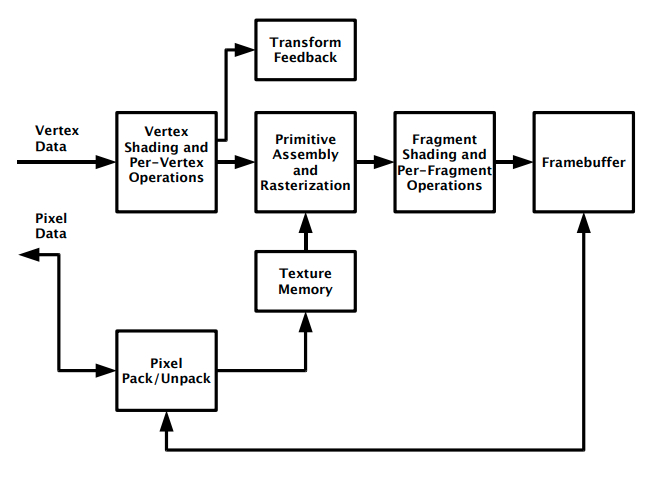
\includegraphics[scale=2.2]{images/chapter2/opengl_pipeline.jpg}
	\caption{Διαδικασία απεικόνισης γραφικών της OpenGL}
	\label{figure:opengl_pipeline}
\end{figure}

\begin{figure}[h]
	\centering
	\begin{subfigure}{.4\textwidth}
		\label{figure:triangle_polyhedron_mesh}
		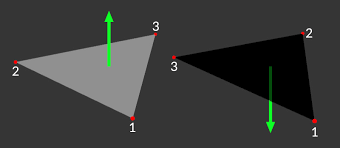
\includegraphics[width=.4\linewidth]{images/chapter2/triangle_normal.png}
		\caption[Πρωτόγονο σχήμα τρίγωνο]{\textsl{Πρωτόγονο σχήμα τρίγωνο}. Φαίνονται οι τρεις κορυφές του τριγώνου καθώς και το κάθετο διάνυσμα στην επιφάνεια του.}
	\end{subfigure}%
	\begin{subfigure}{.4\textwidth}
		\label{figure:dodecahedron}
		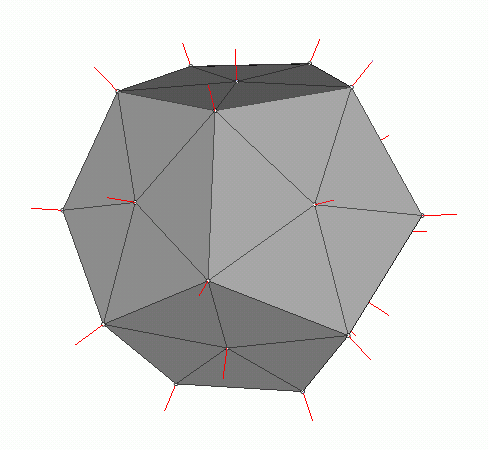
\includegraphics[width=.4\linewidth]{images/appendix/vertex_normal.png}
		\caption[Τρισδιάστατο δωδεκάεδρο πλέγμα]{Τρισδιάστατο δωδεκάεδρο πλέγμα που απαρτίζεται από τρίγωνα.}
	\end{subfigure}
	\caption{Παραδείγματα πρωτόγονων σχημάτων}
\end{figure}


Τα τελικά πρωτόγονα σχήματα περικόπτονται από έναν καθορισμένο όγκο για να προετοιμαστούν για το στάδιο της ψηφιοποίησης. Η διαδικασία αυτή παράγει σειρές από διευθύνσεις του framebuffer συνοδευόμενες από τιμές που περιγράφουν τη δισδιάστατη απεικόνιση των αρχικών τρισδιάστατων πρωτόγονων σχημάτων. Κάθε τμήμα που παράγεται με αυτό τον τρόπο υπόκειται σε περαιτέρω διεργασίες ξεχωριστά. Οι διεργασίες περιλαμβάνουν υπό συνθήκη ενημέρωση των τιμών σε συνάρτηση με εισερχόμενες ή αποθηκευμένες τιμές του βάθους ή του στένσιλ (επιπλέον τιμές που καθορίζουν μετέπειτα επεξεργασία κατά την απεικόνιση), ανάμειξη των εισερχόμενων χρωμάτων με αποθηκευμένα χρώματα ή άλλες διεργασίες στις τιμές των τμημάτων. Τέλος, ο framebuffer επικαιροποιείται με τις τιμές των τμημάτων για κάθε πίξελ, προβάλλοντας έτσι την τελική εικόνα στην οθόνη.